%%%%%%%%%%%%%%%%%%%%%%%%%%%%%%%%%%%%%%%%%%%%%%%%%%%%%%
% Based on THU beamer theme                          %
% Author: EL HASSANI NABIL                           %
% Date: July 2024                                    %
% LPPL Licensed.                                     %
%%%%%%%%%%%%%%%%%%%%%%%%%%%%%%%%%%%%%%%%%%%%%%%%%%%%%%

\documentclass[aspectratio=169]{beamer}
\usepackage[scaled=0.9]{helvet}
\usepackage{courier}
\usepackage[T1]{fontenc}
\usepackage{xcolor,calligra}
\usepackage{graphicx,pstricks,listings,stackengine}
\usepackage{inputenx}
\usepackage{verbatim}
\usepackage{tikz}
\usepackage{calc}

   
\usepackage{UoWstyle}

\titlegraphic{
\includegraphics[height=1.5cm]{pic/efrei_logo.png}}


%==========================================================
\begin{document}
%==========================================================
% Page de titre
\begin{frame}
    \titlepage
\end{frame}

% Plan de la présentation
\begin{frame}
    \frametitle{Plan de la Présentation}
    \scriptsize
    \tableofcontents[hideallsubsections]
\end{frame}

%==========================================================
\section{Introduction}
    \subsection{Objectifs du Cours}

\begin{frame}{Objectifs du Cours}
    \begin{itemize}
        \item \textbf{Comprendre} les concepts fondamentaux des \textbf{Design Patterns} en POO.
        \item \textbf{Acquérir} les compétences pour \textbf{identifier} et \textbf{appliquer} les patterns appropriés en fonction des problèmes rencontrés.
        \item \textbf{Développer} la capacité à concevoir des logiciels \textbf{flexibles}, \textbf{réutilisables} et \textbf{maintenables}.
        \item \textbf{Maîtriser} les patterns les plus courants tels que \textbf{Singleton}, \textbf{Factory}, \textbf{Adapter}, \textbf{Observer}, \textbf{Strategy}.
    \end{itemize}
\end{frame}    
    \subsection{Pourquoi les Design Patterns ?}

\begin{frame}{Pourquoi étudier les Design Patterns ?}
    \begin{itemize}
        \item \textbf{Réutilisation} de solutions éprouvées.
        \item \textbf{Amélioration} de la communication entre développeurs.
        \item \textbf{Facilitation} de la maintenabilité et de l'évolution du code.
        \item \textbf{Renforcement} de la flexibilité et de la modularité des applications.
    \end{itemize}
\end{frame}

%==========================================================

\section{Historique des Design Patterns}
\begin{frame}{Origines des Design Patterns}
    \begin{columns}
        \begin{column}{0.6\textwidth}
            \begin{itemize}
                \item \textbf{Années 1970} : Introduction du concept de "patterns" par \textbf{Christopher Alexander}, architecte.
                \item \textbf{Application en informatique} : Les idées d'Alexander sont adaptées au développement logiciel.
                \item \textbf{1994} : Publication du livre \textit{"Design Patterns: Elements of Reusable Object-Oriented Software"}.
            \end{itemize}
        \end{column}
        \begin{column}{0.4\textwidth}
            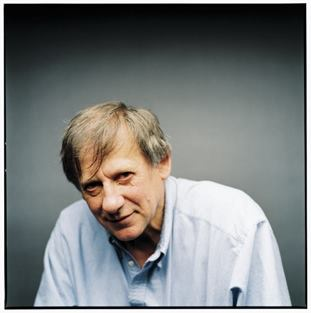
\includegraphics[width=0.8\textwidth]{pic/christopher_alexander.jpg}
            \begin{center}
                \small{\textit{Christopher Alexander}}
            \end{center}
        \end{column}
    \end{columns}
\end{frame}

\begin{frame}{Le Gang of Four (GoF)}
    \begin{columns}
        \begin{column}{0.6\textwidth}
            \begin{itemize}
                \item \textbf{Erich Gamma}
                \item \textbf{Richard Helm}
                \item \textbf{Ralph Johnson}
                \item \textbf{John Vlissides}
            \end{itemize}
            \pause
            \begin{itemize}
                \item Leur livre a profondément influencé la conception logicielle.
                \item A établi un vocabulaire commun pour les développeurs.
                \item A favorisé la diffusion des bonnes pratiques en POO.
            \end{itemize}
        \end{column}
        \begin{column}{0.4\textwidth}
            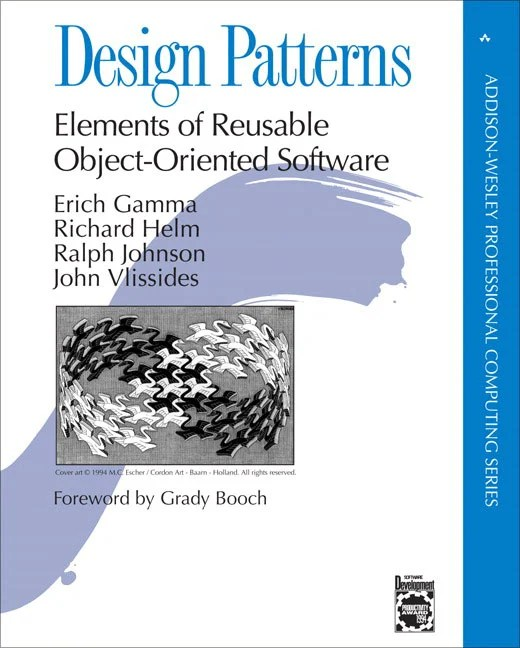
\includegraphics[width=0.9\textwidth]{pic/gof_book.jpg}
            \begin{center}
                \small{\textit{Couverture du livre du GoF}}
            \end{center}
        \end{column}
    \end{columns}
\end{frame}

%==========================================================
%==========================================================

\section{Pourquoi les Design Patterns ?}

\subsection{Des solutions réutilisables aux problèmes récurrents}

\begin{frame}{Des solutions réutilisables aux problèmes récurrents}
    \begin{columns}
        \begin{column}{0.6\textwidth}
            \begin{itemize}
                \item \textbf{Standardisation} des solutions pour des problèmes connus.
                \item \textbf{Gain de temps} : Évite de "réinventer la roue".
                      \pause
                \item \textbf{Exemple} : Le \textbf{Singleton} pour garantir une seule instance d'une classe.
            \end{itemize}
        \end{column}
        \begin{column}{0.4\textwidth}
            \begin{center}
                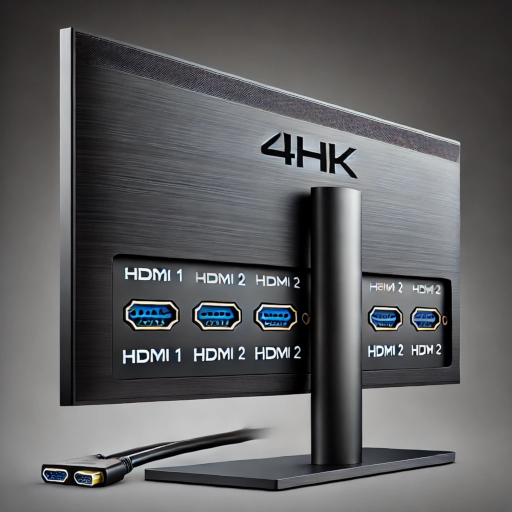
\includegraphics[width=0.8\textwidth]{pic/singleton_pattern.png}
            \end{center}
        \end{column}
    \end{columns}
\end{frame}

\subsection{Amélioration de la communication}

\begin{frame}{Amélioration de la communication}
    \begin{columns}
        \begin{column}{0.6\textwidth}
            \begin{itemize}
                \item \textbf{Vocabulaire commun} facilitant les échanges.
                \item \textbf{Clarté} dans la documentation et le code.
                      \pause
                \item \textbf{Exemple} : "Utilisons un \textbf{Factory Method} ici."
            \end{itemize}
        \end{column}
        \begin{column}{0.4\textwidth}
            \begin{center}
                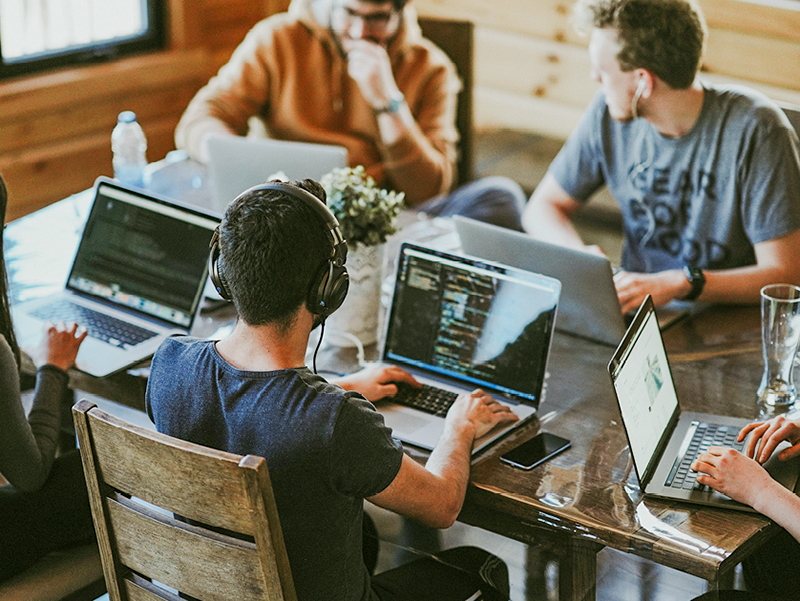
\includegraphics[width=0.8\textwidth]{pic/communication.png}
            \end{center}
        \end{column}
    \end{columns}
\end{frame}

\subsection{Facilitation de la maintenabilité et de l'évolution du code}
\begin{frame}{Facilitation de la maintenabilité et de l'évolution du code}
    \begin{columns}
        \begin{column}{0.6\textwidth}
            \begin{itemize}
                \item \textbf{Code modulaire} et \textbf{flexible}.
                \item \textbf{Facilité} d'ajout de nouvelles fonctionnalités.
                      \pause
                \item \textbf{Exemple} : Le \textbf{Decorator} pour ajouter des responsabilités dynamiquement.
            \end{itemize}
        \end{column}
        \begin{column}{0.4\textwidth}
            \begin{center}
                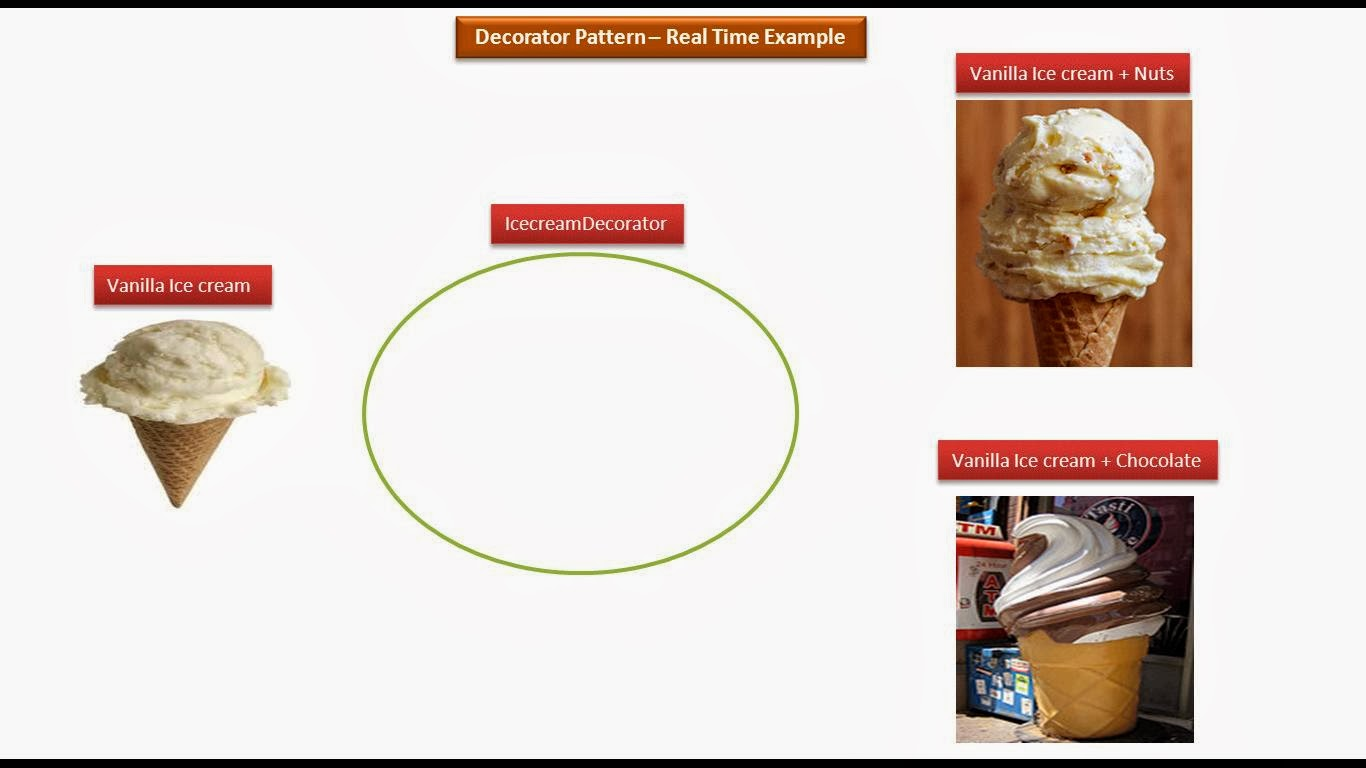
\includegraphics[width=1.0\textwidth]{pic/decorator_pattern.png}
            \end{center}
        \end{column}
    \end{columns}
\end{frame}
\subsection{Renforcement de la flexibilité et de la modularité}

\begin{frame}{Renforcement de la flexibilité et de la modularité}
    \begin{columns}
        \begin{column}{0.6\textwidth}
            \begin{itemize}
                \item \textbf{Séparation des préoccupations}.
                \item \textbf{Interopérabilité} entre les composants.
                      \pause
                \item \textbf{Exemple} : Le \textbf{Adapter} pour faire collaborer des interfaces incompatibles.
            \end{itemize}
        \end{column}
        \begin{column}{0.4\textwidth}
            \begin{center}
                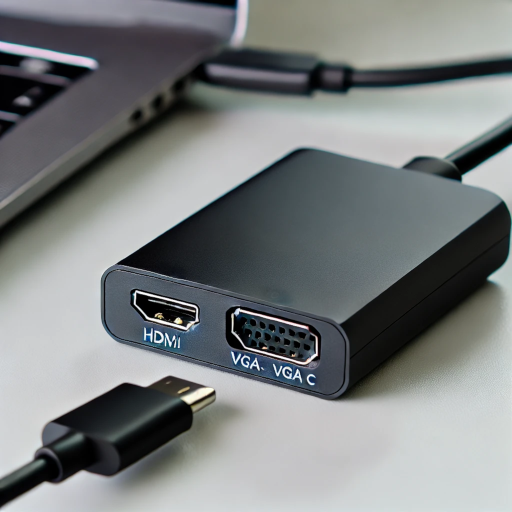
\includegraphics[width=0.8\textwidth]{pic/adapter_pattern.png}
            \end{center}
        \end{column}
    \end{columns}
\end{frame}

%==========================================================
%==========================================================

\section{Catégories de Design Patterns}

\begin{frame}{Catégories de Design Patterns}
    \begin{columns}
        \begin{column}{0.5\textwidth}
            \onslide<1>{
                \centering
                \par Il existe trois grandes catégories de design patterns
            }
            \begin{itemize}
                \item<2-> \textbf{Créationnels :} Concernent la manière dont les objets sont créés.
                \item<3-> \textbf{Structurels :} Traitent de l'organisation des classes et des objets, ainsi que de leurs relations.
                \item<4-> \textbf{Comportementaux :} Concernent l'interaction et la communication entre objets.
            \end{itemize}
        \end{column}
        \begin{column}{0.5\textwidth}
            \only<1>{
                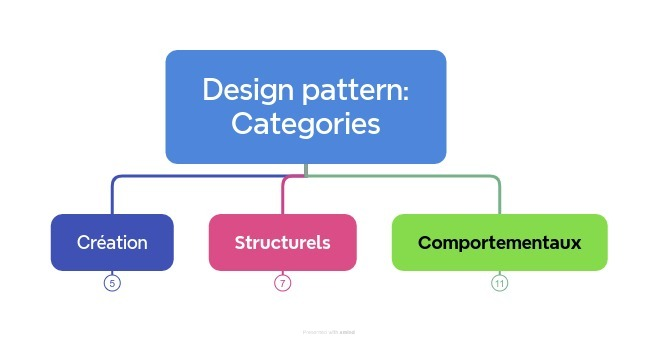
\includegraphics[width=\textwidth]{pic/design_patterns_categories.jpg}
            }
            \only<2>{
                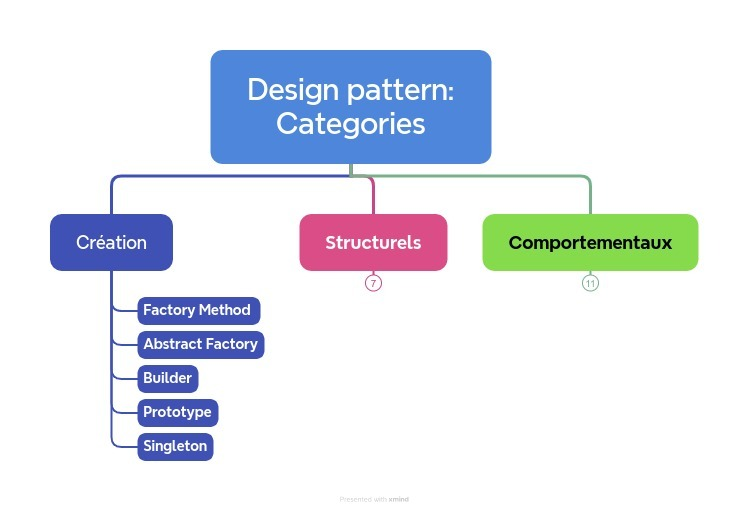
\includegraphics[width=\textwidth]{pic/dep_categorie_2.jpg}
            }
            \only<3>{
                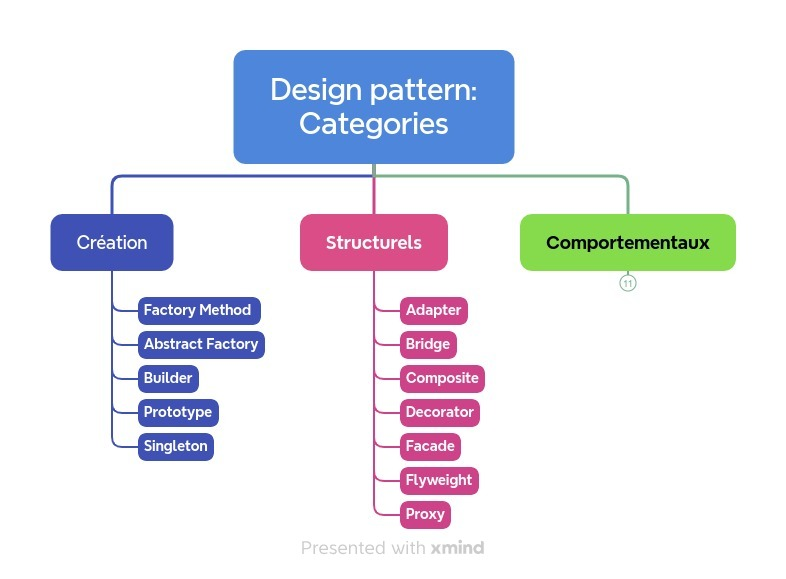
\includegraphics[width=\textwidth]{pic/dep_categorie_3.jpg}
            }
            \only<4>{
                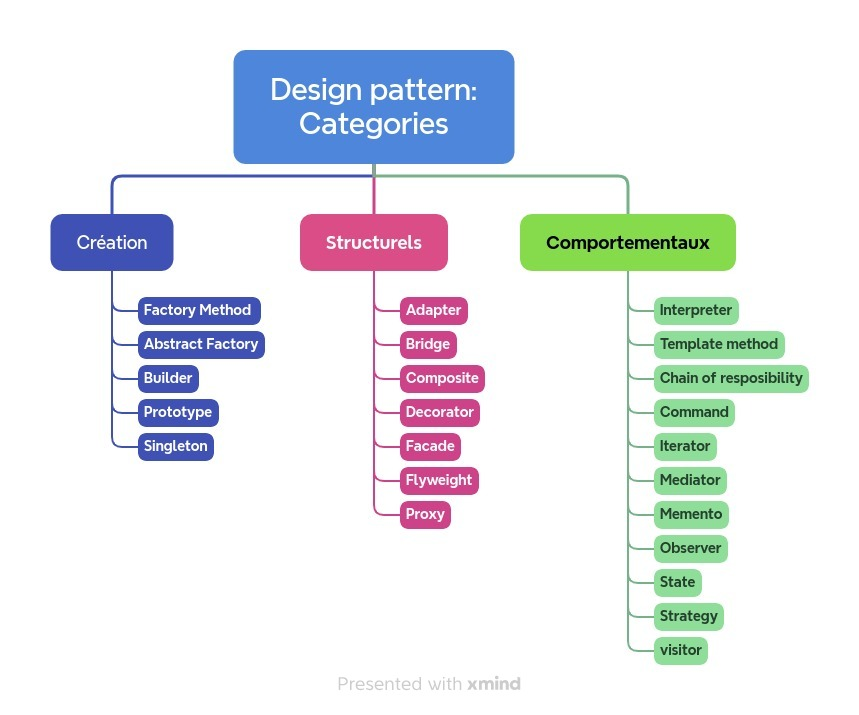
\includegraphics[width=\textwidth]{pic/dep_categorie_4.jpg}
            }
        \end{column}
    \end{columns}
\end{frame}

\begin{frame}{Description des Design Patterns}
    \begin{itemize}
        \item \textbf{Nom du pattern :}
        \begin{itemize}
            \item Le nom unique et concis qui identifie le design pattern.
        \end{itemize}

        \item \textbf{But (Intent) :}
        \begin{itemize}
            \item Une brève description de ce que le pattern fait et pourquoi il est utile.
        \end{itemize}

        \item \textbf{Problème :}
        \begin{itemize}
            \item Le contexte ou la situation récurrente qui nécessite ce pattern.
            \item Les circonstances qui conduisent à l'application de ce pattern.
        \end{itemize}

        \item \textbf{Conséquences :}
        \begin{itemize}
            \item Les avantages à utiliser ce pattern.
            \item Les inconvénients potentiels ou compromis à prendre en compte.
        \end{itemize}
    \end{itemize}
\end{frame}
%==========================================================

\section{Rappel des Fondamentaux de la POO}

\subsection{Principes de la Programmation Orientée Objet}

\begin{frame}{Principes de la Programmation Orientée Objet}
    \begin{columns}
        \begin{column}{0.6\textwidth}
            \begin{itemize}
                \item \textbf{Encapsulation} : Regrouper les données et les méthodes.
                \item \textbf{Abstraction} : Cacher la complexité et ne montrer que l'essentiel.
                \item \textbf{Héritage} : Réutiliser le code en créant des sous-classes.
                \item \textbf{Polymorphisme} : Utiliser une interface commune pour des actions différentes.
            \end{itemize}
        \end{column}
        \begin{column}{0.4\textwidth}
            \pause
            \begin{center}
                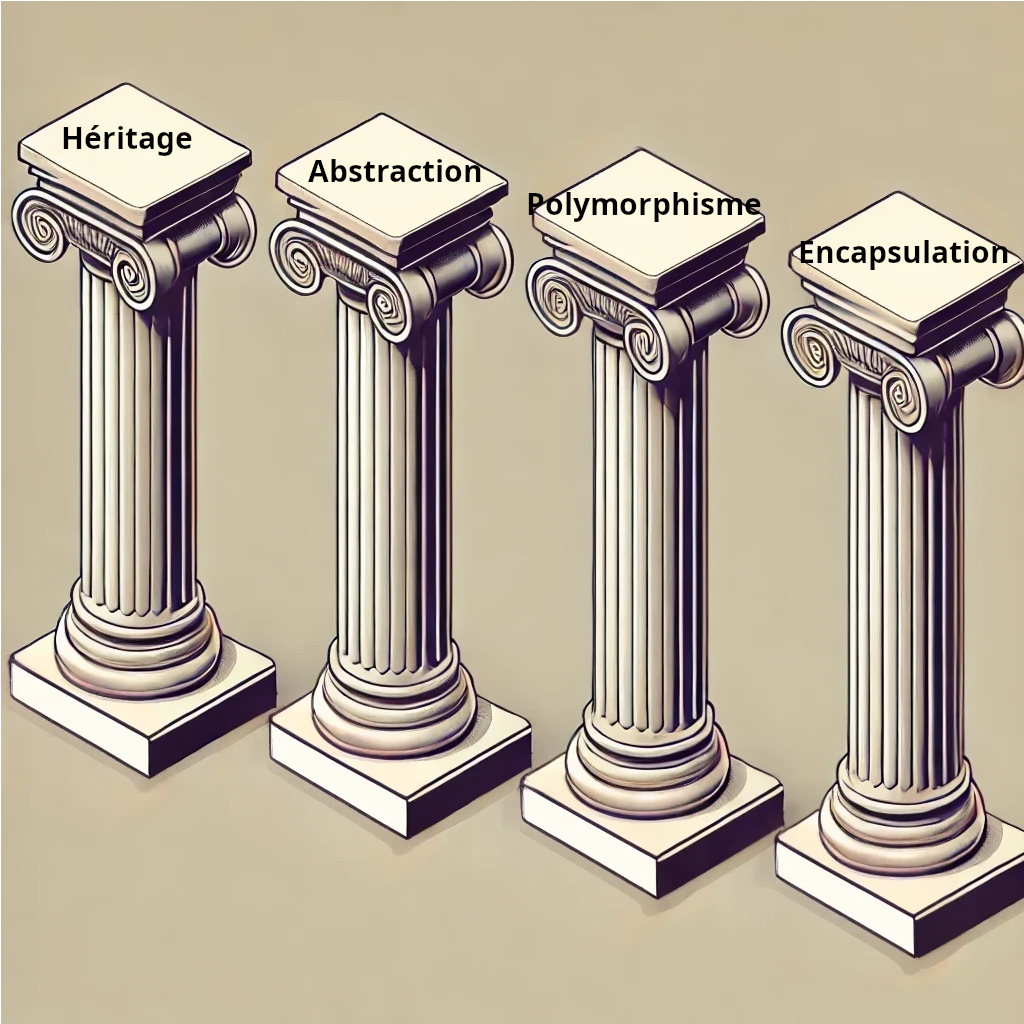
\includegraphics[width=0.6\textwidth]{pic/poo_principles.png}
            \end{center}
        \end{column}
    \end{columns}
\end{frame}

\subsection{Héritage vs Composition}

\begin{frame}{Comparaison : Héritage vs Composition}
    \begin{itemize}
        \item \textbf{Héritage} (\textit{est-un})
              \begin{itemize}
                  \item Avantages :
                        \begin{itemize}
                            \item Réutilisation du code.
                            \item Simplicité de conception.
                        \end{itemize}
                  \item Inconvénients :
                        \begin{itemize}
                            \item Couplage fort entre classes.
                            \item Rigidité face aux changements.
                        \end{itemize}
              \end{itemize}
        \item \textbf{Composition} (\textit{a-un})
              \begin{itemize}
                  \item Avantages :
                        \begin{itemize}
                            \item Flexibilité.
                            \item Faible couplage.
                        \end{itemize}
                  \item Inconvénients :
                        \begin{itemize}
                            \item Complexité initiale.
                            \item Plus de code à écrire.
                        \end{itemize}
              \end{itemize}
    \end{itemize}
\end{frame}

\begin{frame}{Recommandations}
    \begin{itemize}
        \item \textbf{Privilégier la composition} pour une meilleure flexibilité.
        \item \textbf{Utiliser l'héritage} lorsque les classes ont une relation naturelle de type \textit{est-un}.
        \item \textbf{Exemple UML} :
    \end{itemize}
\end{frame}

%==========================================================

\section{La portée des design patterns}
\begin{frame}
    \centering
    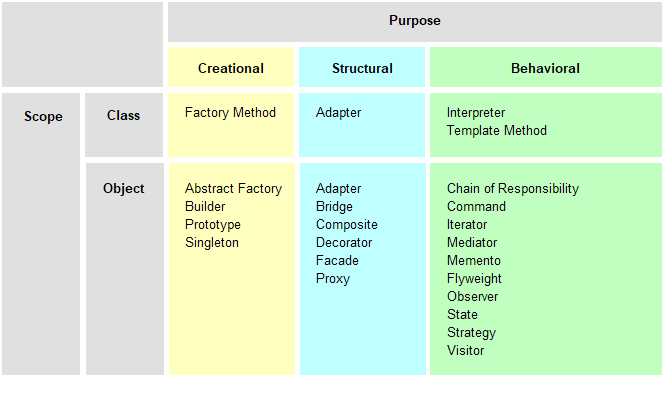
\includegraphics[width=0.9\textwidth]{pic/porte_design_pattern.png}
\end{frame}

\section{Études de Cas et Exemples}
\begin{frame}{Strategy}
    \textbf{Problème :} 
    Comment permettre à un objet de changer dynamiquement son comportement selon des situations différentes, tout en évitant de multiplier les sous-classes.

    \textbf{Solution :} 
    Encapsuler chaque algorithme dans une classe distincte et permettre à l'objet d'interagir avec l'algorithme souhaité via une interface commune.

    \textbf{Cas d'utilisation :}
    Lorsqu'on a plusieurs algorithmes pour accomplir une tâche (par exemple, tri de données) et que l'on veut pouvoir en choisir un au moment de l'exécution.
\end{frame}

% Observer
\begin{frame}{Observer}
    \textbf{Problème :} 
    Comment notifier plusieurs objets d'un changement dans l'état d'un autre objet tout en minimisant les dépendances entre eux.

    \textbf{Solution :} 
    Définir une relation "un à plusieurs" entre des objets : un objet sujet notifie automatiquement tous ses observateurs lorsque son état change.

    \textbf{Cas d'utilisation :}
    Systèmes d'abonnement, comme les interfaces graphiques où plusieurs objets doivent être mis à jour lorsque l'état d'un composant change (ex: modèle-vue-contrôleur).
\end{frame}

% Decorator
\begin{frame}{Decorator}
    \textbf{Problème :} 
    Comment ajouter dynamiquement des fonctionnalités à un objet sans modifier sa structure.

    \textbf{Solution :} 
    Envelopper l'objet original avec un objet décorateur qui ajoute les nouvelles fonctionnalités tout en respectant l'interface de l'objet original.

    \textbf{Cas d'utilisation :}
    Ajout dynamique de fonctionnalités à des composants d'une interface graphique ou à des objets ayant des responsabilités supplémentaires sans changer le code existant.
\end{frame}

% Factory Method
\begin{frame}{Factory Method}
    \textbf{Problème :} 
    Comment créer des objets sans exposer la logique de création et sans lier le code à des classes concrètes.

    \textbf{Solution :} 
    Définir une méthode dans une classe qui délègue la création d'objets aux sous-classes.

    \textbf{Cas d'utilisation :}
    Utilisé lorsqu'un système doit être indépendant du type concret d'objets qu'il doit créer.
\end{frame}

% Singleton
\begin{frame}{Singleton}
    \textbf{Problème :} 
    Comment garantir qu'une classe n'ait qu'une seule instance accessible globalement.

    \textbf{Solution :} 
    Restreindre l'instanciation de la classe à une seule instance et fournir un point d'accès global à cette instance.

    \textbf{Cas d'utilisation :}
    Lorsqu'une seule instance d'une classe est requise, comme un gestionnaire de base de données ou un registre de configuration.
\end{frame}

% Command
\begin{frame}{Command}
    \textbf{Problème :} 
    Comment encapsuler une demande en tant qu'objet, permettant ainsi de paramétrer des actions et de traiter des requêtes de manière flexible.

    \textbf{Solution :} 
    Encapsuler les demandes sous forme d'objets distincts qui peuvent être paramétrés et exécutés.

    \textbf{Cas d'utilisation :}
    Systèmes de gestion des actions (comme les undo/redo), files d'attente de tâches, ou macro-commandes.
\end{frame}

% Adapter
\begin{frame}{Adapter}
    \textbf{Problème :} 
    Comment faire collaborer des interfaces incompatibles de manière transparente.

    \textbf{Solution :} 
    Convertir l'interface d'une classe en une autre interface attendue par le client, afin de rendre des classes incompatibles utilisables ensemble.

    \textbf{Cas d'utilisation :}
    Utilisé lorsqu'un ancien système doit interagir avec un nouveau système aux interfaces différentes.
\end{frame}

% Façade
\begin{frame}{Façade}
    \textbf{Problème :} 
    Comment simplifier l'accès à un ensemble complexe de classes et d'API.

    \textbf{Solution :} 
    Fournir une interface simplifiée à un sous-système complexe.

    \textbf{Cas d'utilisation :}
    Utilisé pour masquer la complexité des systèmes sous-jacents, comme les bibliothèques ou frameworks complexes (ex: interfaces graphiques, bibliothèques de bases de données).
\end{frame}

% Template Method
\begin{frame}{Template Method}
    \textbf{Problème :} 
    Comment définir le squelette d'un algorithme tout en permettant aux sous-classes d'en redéfinir certaines étapes.

    \textbf{Solution :} 
    Implémenter le squelette de l'algorithme dans une méthode de classe parent, tout en permettant aux sous-classes d'implémenter des détails spécifiques.

    \textbf{Cas d'utilisation :}
    Utilisé lorsque plusieurs classes partagent une logique générale, mais certaines étapes doivent être définies au niveau des sous-classes.
\end{frame}

% State
\begin{frame}{State}
    \textbf{Problème :} 
    Comment changer dynamiquement le comportement d'un objet en fonction de son état interne.

    \textbf{Solution :} 
    Encapsuler les états possibles d'un objet dans des classes distinctes, et permettre à l'objet de déléguer son comportement à l'état actuel.

    \textbf{Cas d'utilisation :}
    Utilisé lorsque les objets doivent changer leur comportement en fonction de leur état, comme les machines à états (ex: automate à boisson).
\end{frame}

% Proxy
\begin{frame}{Proxy}
    \textbf{Problème :} 
    Comment contrôler l'accès à un objet en insérant un substitut qui peut gérer les accès.

    \textbf{Solution :} 
    Fournir un proxy qui agit comme un intermédiaire pour contrôler l'accès à l'objet réel, permettant ainsi un contrôle plus fin.

    \textbf{Cas d'utilisation :}
    Utilisé pour gérer l'accès à des objets coûteux à instancier (ex: objets distants, objets à la demande).
\end{frame}

\subsection{Exercice Pratique}

\begin{frame}{Exercice Pratique}
    \textbf{Scénario} : Vous développez une application de messagerie. Lorsqu'un nouvel utilisateur s'inscrit, tous les services associés (profil, notifications, emails) doivent être informés.

    \vspace{0.5cm}

    \textbf{Question} : Quel design pattern utiliseriez-vous pour implémenter cette fonctionnalité, et comment ?

    \vspace{0.5cm}

    \pause

    \textbf{Réponse attendue} : Utilisation du \textbf{Pattern Observer} pour que les services s'abonnent aux événements d'inscription.
\end{frame}

%==========================================================
%==========================================================

\section{Ressources et Références}

\begin{frame}{Ressources et Références}
    \begin{itemize}
        \item \textbf{Livres} :
              \begin{itemize}
                  \item \textit{Design Patterns: Elements of Reusable Object-Oriented Software} - GoF
                  \item \textit{Head First Design Patterns} - Eric Freeman et al.
              \end{itemize}
        \item \textbf{Sites Web} :
              \begin{itemize}
                  \item \href{https://refactoring.guru/design-patterns}{Refactoring Guru}
                  \item \href{https://www.tutorialspoint.com/design_pattern/index.htm}{TutorialsPoint - Design Patterns}
              \end{itemize}
        \item \textbf{Communautés} :
              \begin{itemize}
                  \item \href{https://stackoverflow.com}{Stack Overflow}
                  \item \href{https://www.meetup.com/topics/softwaredev/}{Meetup - Software Development}
              \end{itemize}
    \end{itemize}
\end{frame}

%==========================================================
\begin{frame}{Questions ?}
    \begin{center}
        {\Huge\calligra Merci !}

        \vspace{1cm}

        \Large{Des questions ou des commentaires ?}

        \vspace{0.5cm}

        \small{Vous pouvez me contacter à : \href{mailto:votre.email@efrei.fr}{votre.email@efrei.fr}}
    \end{center}
\end{frame}
%==========================================================

\section{Annexe}
\subsection{Tableau Comparatif des Catégories de Design Patterns}
\begin{frame}{Catégorie : Créationnels}
    \begin{table}[]
        \centering
        \begin{tabular}{|c|p{8cm}|}
            \hline
            \textbf{Design Pattern} & \textbf{Description}                                                                 \\ \hline
            Factory Method          & Définit une méthode pour créer un objet sans spécifier la classe exacte de l'objet.  \\ \hline
            Abstract Factory        & Permet la création de familles d'objets liés sans spécifier leurs classes concrètes. \\ \hline
            Builder                 & Sépare la construction d'un objet complexe de sa représentation.                     \\ \hline
            Prototype               & Crée de nouveaux objets en clonant un prototype existant.                            \\ \hline
            Singleton               & Garantit qu'une classe n'a qu'une seule instance et fournit un point d'accès global. \\ \hline
        \end{tabular}
        \caption{Design Patterns Créationnels}
    \end{table}
\end{frame}

\begin{frame}{Catégorie : Structurels}
    \begin{table}[]
        \centering
        \begin{tabular}{|c|p{8cm}|}
            \hline
            \textbf{Design Pattern} & \textbf{Description}                                                                           \\ \hline
            Adapter                 & Permet de faire fonctionner ensemble des classes qui n'ont pas d'interfaces compatibles.       \\ \hline
            Bridge                  & Sépare l'abstraction de son implémentation pour les développer indépendamment.                 \\ \hline
            Composite               & Compose des objets en structures arborescentes pour représenter des hiérarchies "partie-tout". \\ \hline
            Decorator               & Ajoute dynamiquement des comportements à un objet sans modifier sa structure.                  \\ \hline
            Facade                  & Fournit une interface simplifiée à un ensemble de classes ou un sous-système complexe.         \\ \hline
        \end{tabular}
        \caption{Design Patterns Structurels}
    \end{table}
\end{frame}

\begin{frame}{Catégorie : Comportementaux}
    \begin{table}[]
        \centering
        \begin{tabular}{|c|p{8cm}|}
            \hline
            \textbf{Design Pattern} & \textbf{Description}                                                                           \\ \hline
            Chain of Responsibility & Transmet une requête le long d'une chaîne d'objets jusqu'à ce que l'un la traite.              \\ \hline
            Command                 & Encapsule une requête en tant qu'objet, permettant de paramétrer les actions à effectuer.      \\ \hline
            Iterator                & Permet de parcourir les éléments d'une collection sans exposer sa représentation sous-jacente. \\ \hline
            Observer                & Définit une dépendance entre objets pour notifier automatiquement les changements d'état.      \\ \hline
            Strategy                & Définit une famille d'algorithmes, encapsule chacun et rend les algorithmes interchangeables.  \\ \hline
        \end{tabular}
        \caption{Design Patterns Comportementaux}
    \end{table}
\end{frame}

\end{document}